\documentclass[runningheads]{llncs}
\usepackage[T1]{fontenc}
\usepackage[utf8]{inputenc}
\usepackage[english]{babel}
\usepackage{amsmath}
\usepackage{amssymb}
\usepackage{url}
\usepackage{graphicx}
\usepackage{booktabs}
\usepackage{bbm}
\usepackage{float}

\title{Image Annotation Tool for Dataset Generation and Export with Specialist Training}

\titlerunning{DLA Annotation and Dataset Tool}

\author{Pedro da Rosa\inst{1} \and
Augusto Reich\inst{1} \and
Felipe Zeiser\inst{1} \and
Gabriel Ramos\thanks{gdoramos@unisinos.br}\inst{1}
}
\authorrunning{P. da Rosa et al.}
\institute{Graduate Program in Applied Computing, Universidade Do Vale Do Rio dos Sinos
\email{\{pedrorosa10@edu.,reichaugusto@edu., felipezeiser@, gdoramos@\}unisinos.br}}


\begin{document}
\maketitle

\begin{abstract}
Supervised models in computer vision depend on annotated data; in medical imaging, for example, bottlenecks include specialist time, labeling cost, and scarce annotators~\cite{willemink2020preparing,esteva2017dermatologist}. Established annotation tools prioritize dataset production but rarely integrate, in the same interface, data literacy, supervisor-validated labeling practice, performance metrics, and export to training formats. We present the Data Labelling App (DLA), whose main contribution is that integrated workflow: classification, object detection, and segmentation with assisted practice, automatic grading, free practice, and asynchronous export, backed by a reference \emph{backend}. Annotation and feedback constitute learning activities; validated labels can feed educational citizen-science-style dataset generation under supervisor oversight. We formalize intersection-over-union scoring, Hungarian matching, and grading with \emph{precision}, \emph{recall}, and \emph{F1}. We report exploratory evidence from a pilot cohort ($N=18$) and teacher-dashboard aggregates, without causal claims about learning. We contribute: \emph{(i)} an interface uniting data literacy and dataset generation with geometric feedback; \emph{(ii)} a reproducible evaluation \textit{pipeline}; \emph{(iii)} export to ZIP with COCO metadata and/or YOLO labels from registered datasets. Routes for Kaggle publication can be extended; automated assembly of \emph{new} datasets solely from cohort aggregates, with institutional curation, remains out of scope.

\keywords{computer vision \and data annotation \and educational systems \and machine learning datasets \and medical education.}
\end{abstract}
\section{Introduction}

In contemporary society, advances in artificial intelligence (AI) and computer vision are undeniable. At the core of these technologies lies a critical dependency: the shortage of annotated data, which is essential for training models. In more demanding settings, such as medical imaging domains, expert review requires burdensome curation, inter-annotator variability, and challenges in preparing data for machine learning~\cite{willemink2020preparing}; in chest radiography, for instance, reference datasets still illustrate uncertainty among expert readers~\cite{irvin2019chexpert}. Producing these labels requires knowledge that is only sparsely available to non-experts. Thus, obtaining this kind of annotation typically requires a specialist.

Therefore, a tension arises: models need data to tackle complex tasks, yet experienced annotators are needed to make that feasible. In other words, both specialists and annotated data are indispensable. Data annotation tends to be costly in time and resources and is often among the most labor-intensive components in developing machine learning systems, as summarized in domain reviews~\cite{willemink2020preparing}.

The literature offers many data annotation tools, including academic initiatives such as the VGG Image Annotator (VIA)~\cite{dutta2019via}. However, they still depend on specialists. Conversely, formal education often lacks practical tools aligned with the role of humans in interactive learning cycles~\cite{amershi2014power}.

In this paper, we present the Data Labelling App (DLA). Under \emph{supervisor}\footnote{In the DLA workflow, \emph{supervisor} and \emph{annotator} denote the platform roles corresponding to the classroom \emph{teacher} and \emph{student}, respectively.} oversight, assisted practice yields graded feedback; free practice extends labeling without immediate scoring; routine activity can produce exportable \textit{datasets} in formats such as COCO~\cite{lin2014microsoft} and YOLO~\cite{ultralytics}, subject to institutional curation. Design, functionality, and reference implementation are detailed in Section~\ref{sec:arquitetura}; grading criteria and pilot-cohort results appear in Section~\ref{sec:res}.

The main contributions of this work are threefold:
\begin{itemize}
    \item We introduce an integrated interface that links data literacy, visual annotation practice, and supervisor-validated feedback in a single pedagogical workflow.
    \item We formalize an automatic \textit{pipeline} with IoU, Hungarian matching, and \emph{F1} scoring to grade annotator submissions, with \emph{precision} and \emph{recall} in the scoring flow.
    \item We implement export that generates, through routine pedagogical use, structured \textit{datasets} in {COCO}~\cite{lin2014microsoft} and {YOLO} formats, contributing validated labels where annotated data are scarce, subject to supervisor curation outside the classroom.
\end{itemize}

Existing tools seldom address, in one interface, the joint shortage of annotated data in many sciences~\cite{willemink2020preparing,esteva2017dermatologist} and limited \emph{data literacy} among learners, the ability to demarcate, label, and visually verify images in domains where that competence is required~\cite{wolff2016data,pangrazio2019personal}. DLA is not a tutorial on how to annotate; its contribution is the integrated interface that couples pedagogical practice with validated dataset generation under supervisor feedback, in line with educational citizen-science models~\cite{wiggins2011citizen}. Annotation and automated or manual feedback are learning activities in themselves; when a supervisor later uses exported data, those labels may also support downstream uses such as training vision models.

\section{Related work}

Many tools support data annotation, especially in computer vision. They play a fundamental role in creating labeled sets, which are essential for training machine learning models.

Among the more complete solutions, CVAT~\cite{cvat} appears frequently in recent work, above all for its flexibility: it supports different annotation types, such as detection, segmentation, and classification, and organizes tasks and datasets in a relatively structured way. Another advantage is support for formats such as COCO and YOLO, which facilitates direct use of the data in training pipelines.

Labelbox~\cite{labelbox} follows a similar line but with greater emphasis on large-scale use. The platform prioritizes collaboration and project management, which is appropriate when many people annotate in parallel. On the other hand, as a commercial solution, it is not always viable in academic contexts or smaller projects.

Tools such as LabelMe~\cite{russell2008labelme} and LabelImg~\cite{labelimg} are simpler and are often adopted in more specific settings. LabelMe is commonly associated with polygon- or region-based segmentation; LabelImg is straightforward and oriented to bounding boxes (\emph{bounding boxes}). Although easy to use, they offer less support for organizing \textit{datasets} and integrating multiple formats, which limits more complex applications.

More recently, mature platforms such as CVAT and Labelbox have added AI-assisted pre-labeling, active-learning workflows, and human-in-the-loop review to reduce annotation effort at scale. These techniques represent the current state of the art in data annotation pipelines: AI-assisted labeling uses machine learning models to generate initial annotations, while active learning prioritizes the most informative samples for human review, reducing overall labeling effort. Table~\ref{tab:ferramentas} summarizes both classic export and pedagogical features and this newer axis; DLA does not target model-assisted labeling, but rather pedagogical integration under supervisor-validated practice.

\begin{table}[t]
  \centering
  \caption{Summary comparison among annotation tools. Check marks indicate support declared or typical in public documentation; $\sim$ indicates partial or plugin-based support; blank cells indicate absent or very limited support.}
  \label{tab:ferramentas}
  % \resizebox{\linewidth}{!}{%
  \begin{tabular}{lccccc}
    \toprule
    \textbf{Feature} & \textbf{DLA} & \textbf{LabelMe} & \textbf{LabelImg} & \textbf{CVAT} & \textbf{Labelbox} \\
    \midrule
    Register \textit{datasets} & \checkmark &  &  & \checkmark & \checkmark \\
    Object classification & \checkmark & \checkmark &  & \checkmark & \checkmark \\
    Object segmentation & \checkmark & \checkmark &  & \checkmark & \checkmark \\
    Object detection & \checkmark &  & \checkmark & \checkmark & \checkmark \\
    AI-assisted annotation &  &  &  & \checkmark & \checkmark \\
    Active learning &  &  &  & $\sim$ & \checkmark \\
    Export to Kaggle & \checkmark &  &  &  &  \\
    Export ZIP & \checkmark &  &  & \checkmark & \checkmark \\
    COCO format & \checkmark &  &  & \checkmark & \checkmark \\
    YOLO format & \checkmark &  & \checkmark & \checkmark & \checkmark \\
    Pedagogical monitoring & \checkmark &  &  &  &  \\
    Pedagogical grading & \checkmark &  &  &  &  \\
    \bottomrule
  \end{tabular}%}
\end{table}

Given this landscape, mature annotation options exist, each with advantages depending on context. Nevertheless, these solutions are predominantly oriented to creating \textit{datasets} or reducing labeling effort through AI assistance, without integrating data literacy, supervisor-validated pedagogical practice, and export in the same workflow, the gap DLA targets at the interface level.

\section{System architecture}\label{sec:arquitetura}

This section is organized in two parts: \emph{design and functionality} (what supervisors and annotators do, and how pedagogical flows are structured) and \emph{reference implementation} (the stack deployed in the public repository).

\subsection{Design and functionality}

\subsubsection{Overview and system flow}

In this subsection we present a high-level view of the system and the division of responsibilities among components. Supervisors and administrators access protected routes to create \textit{datasets} and exercises; annotators see exercise listings filtered by class, created and managed by administrators, and submit responses to those exercises. Per image, responses occupy two logical compartments: \texttt{labelledAnswers}, for supervised practice and automatic grading, and \texttt{unlabelledAnswers}, for free practice, without grade recomputation in the described flow. When supervised responses are persisted, the submission use case computes \texttt{supervisedScore} from the dataset identifier and exercise configuration, including IoU thresholds, \emph{F1} or coverage-oriented \emph{recall} mode, and the optional list of supervised media. When an exercise is finalized, completion metadata is recorded and an action log entry is triggered for pedagogical auditing.

The operational flow is as follows: an authenticated supervisor registers \textit{datasets} and exercises; an authenticated annotator submits responses; the server persists submissions, computes the supervised-practice grade when applicable, and exposes data to dashboards where metrics and results can be inspected by supervisors or administrators; labeled data and exercise history can then be exported; long exports are delegated to asynchronous \emph{workers}, tracked by task identifier.

\begin{figure}[t]
    \centering
    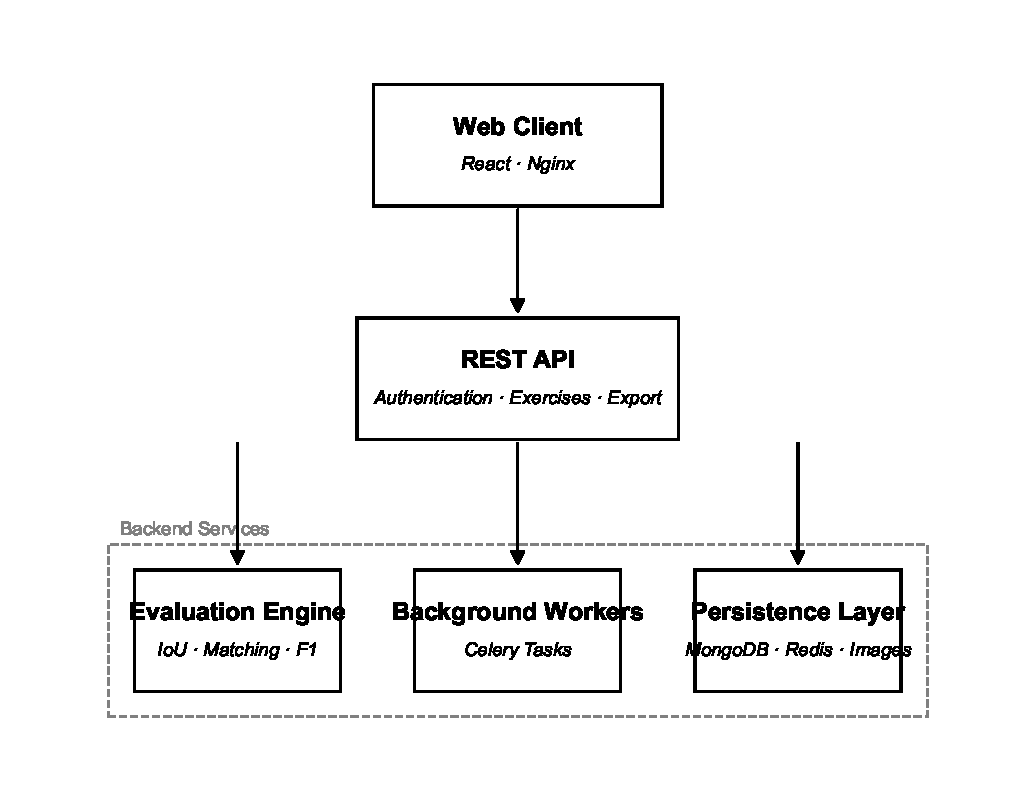
\includegraphics[width=0.96\linewidth]{system_arch_macro.pdf}
    \caption{High-level architecture of the proposed annotation and evaluation platform.}
    \label{fig:arquitetura}
\end{figure}

In summary, Figure~\ref{fig:arquitetura}\footnote{For architectural detail beyond this macro view and access to the complete reference implementation, see the open-source DLA repository at \url{https://github.com/ramos-ai/dla-bracis}.} outlines the chain from client to service to data; the following subsections detail annotation, export, and grading criteria.

\subsubsection{Annotation module}

In this subsection we detail how the system represents annotation tasks, which artifacts the supervisor configures, and how annotator responses are stored to enable automatic grading or export.

The supervisor \textbf{creates exercises} linked to a \textit{dataset} and a task type; each annotator produces an \textbf{exercise submission}, updated over time, composed of per-image \textbf{response submissions}, whether as labels, boxes, or polygons. Each exercise generally combines two modalities. In \textbf{assisted practice}, the system compares responses to the supervisor reference and may update the supervised score \texttt{supervisedScore}; for this, the supervisor must have labeled in advance a subset of images that constitute the assisted exercise. In \textbf{free practice}, the annotator labels any image in the \textit{dataset} without that immediate grading in the same scoring flow. This distinction is \textbf{critical for export}: the pipeline in the next subsection must know which responses count as reliable training labels, typically those from assisted practice and/or finalized submissions, whereas free practice may be excluded or handled separately, for example, through an option to include unlabeled items or curation policies. Ignoring this separation would mix examples without reference or without geometric validation with corrected examples, reducing exported set quality and obscuring the pedagogical reading of the data.

The task type follows the dataset field \texttt{task\_type}, with values \texttt{classification}, \texttt{detection}, or \texttt{segmentation}, and there is additional branching in the scoring service: if responses contain COCO-style annotations with \texttt{annotations} and a \texttt{bbox} bounding-box field, the detection flow is selected even when textual metadata is generic. References are drawn from per-media labels in classification, stored box annotations in detection, and persisted polygons with reference class labels in segmentation. For segmentation, annotators delineate regions with polygon tools in the web client; Figure~\ref{fig:segmentation} illustrates this workflow on a medical image.

\begin{figure}[H]
    \centering
    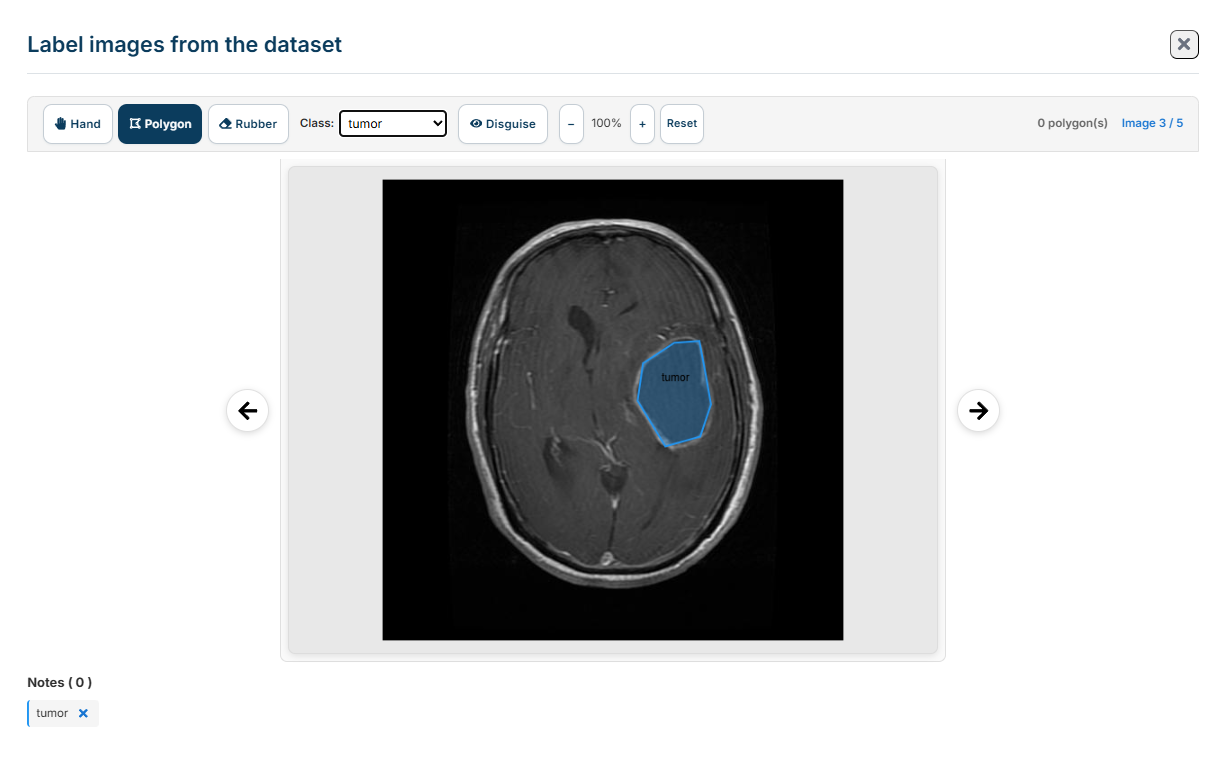
\includegraphics[width=\linewidth,height=0.38\textheight,keepaspectratio]{segmentation_tool.png}
    \caption{Demonstration of the DLA annotation interface for polygon segmentation on a medical image.}
    \label{fig:segmentation}
\end{figure}

Each exercise stores configurable grading parameters: overlap thresholds $\tau$ (possibly distinct for boxes and polygons), a scoring mode based on \emph{F1} or \emph{recall}, an exercise weight applied to raw scores, and the set of images included in supervised-practice averaging; unanswered listed images count as zero in that average.

The supervisor may also apply manual corrections to detection and segmentation submissions via a dedicated route, separate from the automatic grading module, enabling point fixes in specific cases.

For dashboards, the system aggregates, per exercise, completion rate, mean percentage score, and simplified bin histograms for the supervisor, and exposes to the annotator summary indicators such as completed exercises, mean score, and submission count; the supervisor view is illustrated in Figure~\ref{fig:dashboard}.

\subsubsection{Dataset generation pipeline}

In this subsection we describe the \textit{dataset} export pipeline out of the DLA environment, either as a ZIP file or, when configured, as publication to a Kaggle repository, with reproducible parameters and asynchronous execution.

Configuration is performed by the \texttt{ExportConfig} structure: simple or custom mode, percentages or manual assignment of \texttt{train}, \texttt{val}, and \texttt{test} splits, formats \texttt{coco}, \texttt{yolo}, \texttt{both}, or \texttt{auto}, pseudo-random \texttt{seed}, class filters, optional inclusion of unlabeled items, width limits, and JPEG quality. The COCO format follows common detection metadata conventions~\cite{lin2014microsoft}; YOLO-style labels follow folder and text-file conventions compatible with training ecosystems~\cite{ultralytics}.

Long-running export jobs expose progress queryable by task identifier; the completed file is served through an authenticated download route. Optional integration with the Kaggle ecosystem~\cite{kaggle} depends on institutional configuration.

For reproducibility, setting \texttt{seed}, split mode, and format in the export request yields stable partitions across \textit{dataset} generations, unless source data change, for example, through manual image selection.

\subsubsection{Automatic grading module}

In this subsection we formalize the geometric grader used to turn annotator submissions into quantitative feedback aligned with common object detection and instance segmentation practice. Each exercise defines a set of classes, an overlap threshold $\tau \in [0,1]$, and a scoring mode, either \emph{F1} or \emph{recall}. For \emph{classification} items, the module compares the selected label to the reference label and assigns a binary correctness score. The remainder of this subsection concerns \emph{localization} with bounding boxes, i.e., \texttt{bbox} regions or polygons, in detection or segmentation, where geometry and one-to-one matching are essential.

\paragraph{Numerical safeguards.}
To avoid undefined ratios and degenerate regions, we adopt fixed tolerances: a general union-area floor $\varepsilon = 10^{-6}$, an additional floor $\varepsilon_{\mathrm{seg}} = 10^{-9}$ for segmentation stability, and a minimum polygon area $A_{\min}=10^{-8}$; below that threshold, the polygon is ignored. These values match those recorded in the reference source code.

\paragraph{Overlap for boxes and polygons.}
Let a bounding box in \texttt{bbox} format $(x_{\min}, y_{\min}, w, h)$ have area $\mathrm{area}(B)=w\cdot h$. For two boxes, $\mathrm{IoU}(B,B')$, i.e., intersection over union, the usual metric in detection challenges such as PASCAL~VOC~\cite{everingham2010pascal} and COCO-style sets~\cite{lin2014microsoft}, is the ratio of intersection area to union area; if union area is below $\varepsilon$, we set $\mathrm{IoU}=0$.

For a simple polygon with vertices $(x_i,y_i)$ listed in order, the shoelace formula gives
\begin{equation}
\mathrm{area}(P)=\frac{1}{2}\left|\sum_{i=0}^{n-1}\left(x_i y_{i+1}-x_{i+1} y_i\right)\right|,
\end{equation}
with indices taken modulo $n$. Treating two polygons as regions $P,Q \subset \mathbb{R}^2$, mask-style overlap is
\begin{equation}
\mathrm{IoU}(P,Q)=
\begin{cases}
\dfrac{\mathrm{area}(P\cap Q)}{\mathrm{area}(P\cup Q)}, & \text{if } \mathrm{area}(P\cup Q)>\varepsilon_{\mathrm{seg}},\\
0, & \text{otherwise}.
\end{cases}
\end{equation}
For segmentation exercises, an \emph{effective} overlap encourages conservative masks: if the annotator's polygon lies inside the reference region ($P \subseteq Q$), we set $\mathrm{IoU}_{\mathrm{eff}}(P,Q)=1$; otherwise, $\mathrm{IoU}_{\mathrm{eff}}(P,Q)=\mathrm{IoU}(P,Q)$. This metric establishes a \textit{trade-off} between the strictness of computer vision \textit{benchmarks} and pedagogical feasibility: at the learning stage, underestimating area, that is, an inner mask, is treated as a preferable manual precision error to extending beyond the reference polygon. Sensitivity to this criterion is modulated by the supervisor through the threshold $\tau \in [0,1]$, allowing the tool to act as a configurable quality filter before data export.

\paragraph{Optimal matching between annotator and reference objects.}
Let $\mathcal{S}=\{s_1,\dots,s_{N_s}\}$ be objects annotated by the learner and $\mathcal{R}=\{r_1,\dots,r_{N_r}\}$ reference objects in the same image, each with a discrete class label. Only same-class pairs are eligible for matching. Let $\mathrm{IoU}^{\star}(s_i,r_j)$ be standard box IoU in detection tasks and $\mathrm{IoU}_{\mathrm{eff}}$ in polygon segmentation tasks. Define a rectangular cost matrix
\begin{equation}
C_{ij}=
\begin{cases}
1-\mathrm{IoU}^{\star}(s_i,r_j), & \text{if the classes of } s_i \text{ and } r_j \text{ match},\\
+\infty, & \text{otherwise}.
\end{cases}
\end{equation}
The minimum-cost Hungarian algorithm~\cite{kuhn1955hungarian} returns a one-to-one matching $M$ between annotator and reference indices. This prevents multiple learner boxes from collapsing onto a single reference object, a common failure mode of greedy overlap-only matching.

A matched pair $(i,j)\in M$ counts as a true positive only if overlap reaches the exercise threshold:
\begin{equation}
\mathrm{TP}=\sum_{(i,j)\in M}\mathbbm{1}\!\left(\mathrm{IoU}^{\star}(s_i,r_j)\ge \tau\right),
\end{equation}
where $\mathbbm{1}(\cdot)$ is the indicator function. Unmatched annotator objects contribute to false positives and unmatched reference objects to false negatives:
\begin{equation}
\mathrm{FP}=N_s-\mathrm{TP},\qquad \mathrm{FN}=N_r-\mathrm{TP}.
\end{equation}

\paragraph{\emph{Precision}, \emph{recall}, \emph{F1}, and score.}
\emph{Precision} and \emph{recall} (or sensitivity, in the terminology of the field) are expressed in $[0,1]$ as
\begin{equation}
P=\begin{cases}
\dfrac{\mathrm{TP}}{\mathrm{TP}+\mathrm{FP}}, & \text{if } \mathrm{TP}+\mathrm{FP}>0,\\
0, & \text{otherwise},
\end{cases}
\qquad
R=\begin{cases}
\dfrac{\mathrm{TP}}{\mathrm{TP}+\mathrm{FN}}, & \text{if } \mathrm{TP}+\mathrm{FN}>0,\\
0, & \text{otherwise}.
\end{cases}
\end{equation}
The main scalar is the \emph{F1} measure, written directly from counts as
\begin{equation}
\mathrm{F1}=
\begin{cases}
\dfrac{2\,\mathrm{TP}}{2\,\mathrm{TP}+\mathrm{FP}+\mathrm{FN}}, & \text{if } 2\,\mathrm{TP}+\mathrm{FP}+\mathrm{FN}>0,\\
0, & \text{otherwise},
\end{cases}
\end{equation}
which coincides with the harmonic mean of \emph{precision} and \emph{recall}, $2PR/(P+R)$, whenever $P+R>0$. For exercises configured to emphasize coverage, the same flow uses \emph{recall} $R$ to drive the score. Scores on the $0$--$100$ scale are given by $\mathrm{Score}_{\mathrm{F1}}=100\cdot \mathrm{F1}$ or $\mathrm{Score}_{R}=100\cdot R$, according to the educator's configuration.

\paragraph{Degenerate cases.}
If $N_r=N_s=0$, the image contains nothing to mark; the module assigns a neutral maximum score ($100$). If exactly one side is empty ($N_r=0<N_s$ or $N_r>0=N_s$), the result is $0$, indicating spurious objects or complete omission.

\paragraph{End-to-end grading flow.}
In summary, the module (i) computes paired overlaps under class constraints, (ii) builds $C$, (iii) solves for the optimal matching $M$, (iv) applies $\tau$ to obtain $\mathrm{TP}$, $\mathrm{FP}$, and $\mathrm{FN}$, and (v) aggregates $P$, $R$, and $\mathrm{F1}$ into a configurable score. This \textit{pipeline} mirrors standard detection/segmentation evaluation while remaining interpretable for annotators: \emph{precision} answers ``how much of what I drew was correct?'', \emph{recall} answers ``how much of what mattered did I find?'', and \emph{F1} balances the two.

\subsection{Reference implementation}

The public DLA \emph{backend} is implemented as an HTTP API in Flask~\cite{flask}, with persistence in MongoDB~\cite{mongodb}, binary image storage (e.g., via GridFS), evaluation domain logic isolated in pure Python modules, work queues with Celery~\cite{celery}, and observability via Prometheus/Grafana~\cite{prometheus,grafana}. Operational metrics and auditable \textit{logs} support monitoring in deployed settings.

Physical ZIP generation, including resized images when configured, \texttt{dataset.json}, image and label folders, runs in a Celery task with retries, decoupling API response time; routes and tasks also support Kaggle credentials and publication when configured.

In the evaluation domain, logic is isolated in Python modules without a Flask dependency: numeric constants match $\varepsilon$, $\varepsilon_{\mathrm{seg}}$, and $A_{\min}$ above; bounding boxes use analytic intersection in the plane; polygons in normalized coordinates use area via the shoelace formula and mask-style IoU via Shapely~\cite{shapely}; the cost matrix is built in NumPy~\cite{harris2020array}; matching is solved with the Hungarian assignment method~\cite{kuhn1955hungarian}, via SciPy's \texttt{linear\_sum\_assignment} routine~\cite{virtanen2020scipy}. The reader can replicate grading behavior by combining the equations above with the same hyperparameters and libraries.

\section{Results and experiments}\label{sec:res}

This section presents results from a field study with a pilot cohort, indicators from the teacher dashboard, and observations in a staging environment. The design remains descriptive and does not aim at causal inference about learning generalizable to other populations; nevertheless, the findings constitute relevant empirical evidence about platform operation and experience, the teacher dashboard, and performance of a group with a clearly technical profile.

\subsection{Field study with pilot cohort ($N=18$)}

The user test involved 18 authenticated participants ($N=18$), members of a computer science research group, with education ranging from undergraduate to graduate levels. The sample comprised 14 men and 4 women, aged 19 to 65. The test data allow quantifying aggregate performance, exercise completion rates, and usage patterns in a cohort with a defined technical and academic profile. Three exercises were provided for this cohort, one per DLA task type: classification, object detection, and polygon segmentation; each had five images in assisted practice. In the classification exercise, images alternated between two visual domains, wildlife (labels \emph{elephant}, \emph{raccoon}, and \emph{zebra}) and chest radiography (\emph{pneumonia} or \emph{healthy}), without mixing the two families in the same image. The dashboard export, however, produced a single confusion matrix aggregating answer--reference pairs from both domains; Tables~\ref{tab:confusao-fauna} and~\ref{tab:confusao-pulmao} split the view by domain to avoid mistaken interpretations across unrelated classes. For detection and segmentation, an IoU threshold $\tau = 0.75$ and F1-based scoring were adopted to relax grading slightly for cohorts at an early training stage. There was no randomized content assignment across groups nor a formal pre-test; the focus was observing task completion, the grade distribution, and error patterns in classification.

\subsection{Teacher dashboard and exercise performance indicators}

For the analyzed slice, the teacher dashboard (Figure~\ref{fig:dashboard}) showed three registered exercises, eighteen students with recorded activity, and fifty-four submissions counted in the aggregator. The overall mean supervised score was $76.4\,\%$, with an exercise completion rate of $95.5\,\%$. These summary indicators, displayed as \textit{big numbers} in the interface, summarize cohort effort and concentration at high scores, albeit with dispersion across exercises and students.

\begin{figure}[H]
    \centering
    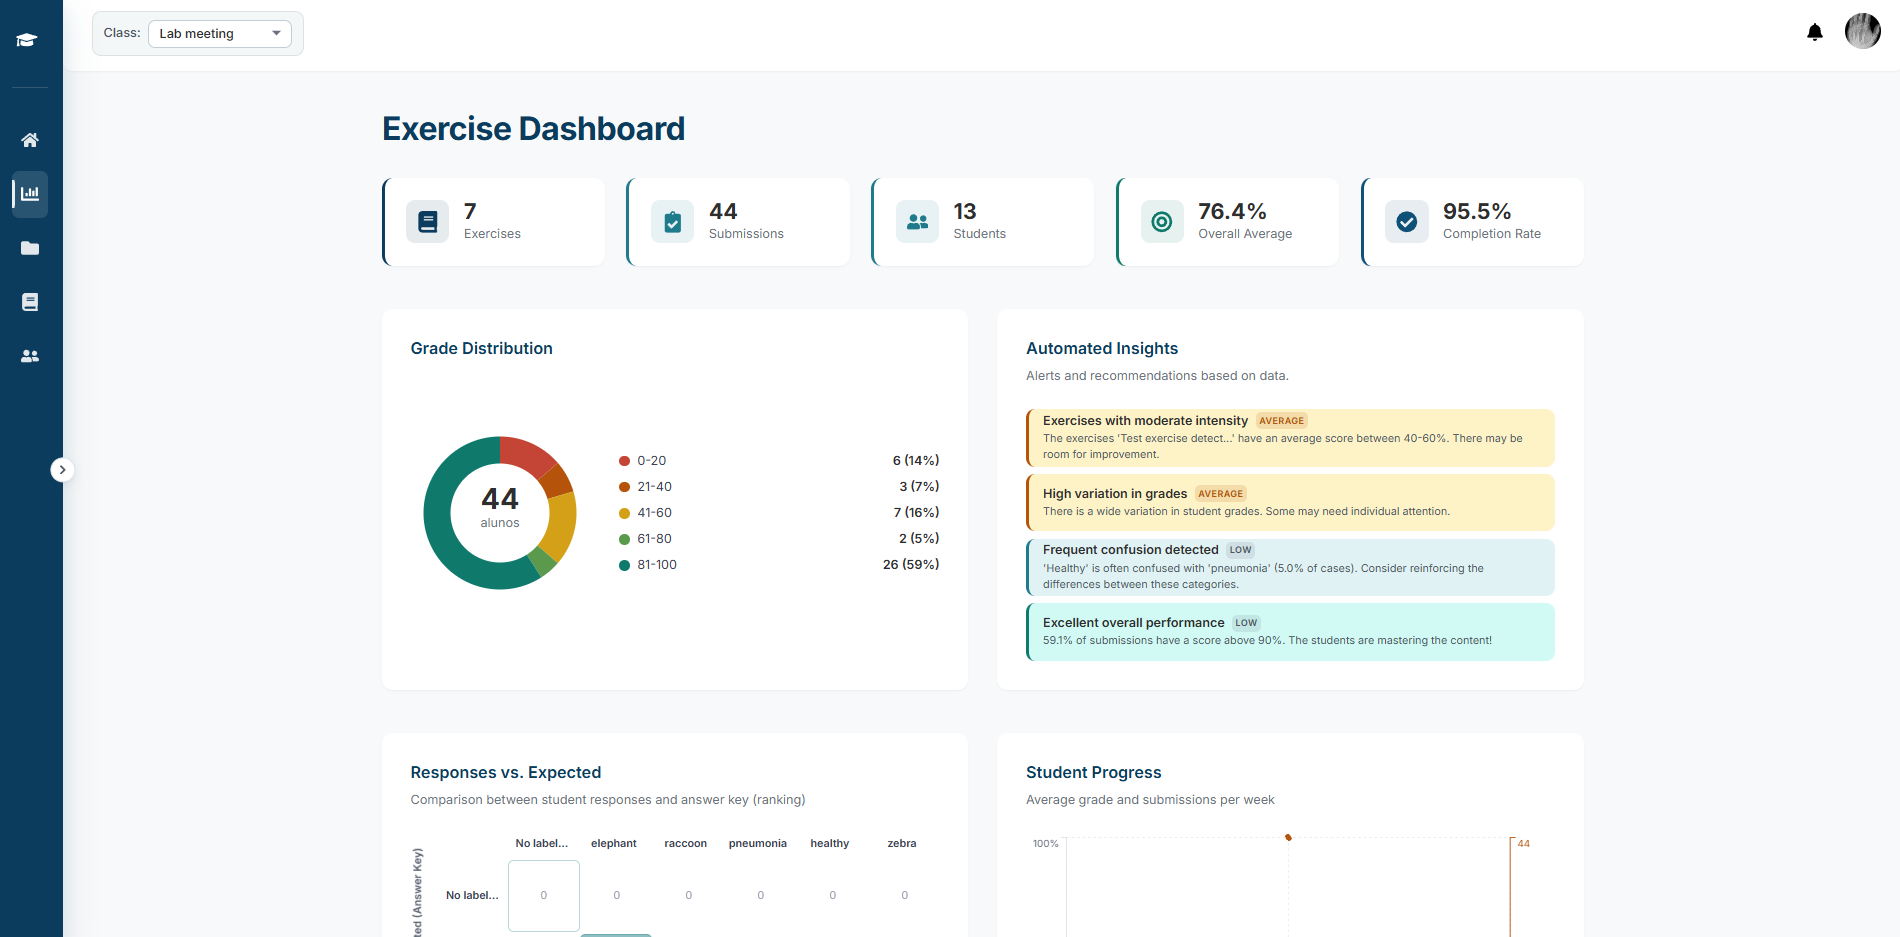
\includegraphics[width=\linewidth]{system_dashboard_screenshot.png}
    \caption{Supervisor exercise dashboard for the pilot cohort: aggregate metrics, grade distribution, automated pedagogical alerts, response--reference confusion matrix, and weekly progress indicators.}
    \label{fig:dashboard}
\end{figure}

\begin{table}[t]
  \centering
  \caption{Aggregate indicators shown on the teacher dashboard for the pilot slice.}
  \label{tab:big-numbers}
  \begin{tabular}{lc}
    \toprule
    Indicator & Value \\
    \midrule
    Exercises considered & 3 \\
    Aggregated submissions & 54 \\
    Students with activity & 18 \\
    Overall mean score & $76.4\,\%$ \\
    Completion rate & $95.5\,\%$ \\
    \bottomrule
  \end{tabular}
\end{table}

Beyond the totals in Table~\ref{tab:big-numbers} and the interface layout in Figure~\ref{fig:dashboard}, the dashboard emitted descriptive alerts, one of the educator dashboard features, including: high dispersion among individual scores, suggesting possible need for follow-up; recurrent confusion between the \emph{healthy} and \emph{pneumonia} classes, cited in about $5\,\%$ of cases analyzed by the dashboard; and, in contrast, a large fraction of submissions above $90\,\%$, about $69\,\%$ of the total in Table~\ref{tab:notas-faixas}, compatible with a simple taxonomic domain or a rapid training effect in the pilot classification, which gives the teacher a favorable view of student progress on that classification task.

\begin{table}[H]
  \centering
  \caption{Empirical grade distribution by bin, with $n=54$ submissions. Using bin midpoints, $\sum_i n_i m_i / n = 4120/54 \approx 76.3\,\%$.}
  \label{tab:notas-faixas}
  \begin{tabular}{lcc}
    \toprule
    Grade bin (\%) & Submissions & Fraction \\
    \midrule
    $0$--$20$   & 3  & $6\,\%$ \\
    $21$--$40$  & 3  & $6\,\%$ \\
    $41$--$60$  & 5  & $9\,\%$ \\
    $61$--$80$  & 6  & $11\,\%$ \\
    $81$--$100$ & 37 & $69\,\%$ \\
    \bottomrule
  \end{tabular}
\end{table}

Table~\ref{tab:notas-faixas} summarizes the empirical grade distribution by percentage bins over the fifty-four submissions; bin counts were reconciled with the dashboard global mean of $76.4\,\%$ using bin midpoints $10$, $30$, $50$, $70$, and $90$, implying $\sum_i n_i m_i / n = 4120/54 \approx 76.3\,\%$; the small gap is attributable to integer rounding.


For the classification exercise, Tables~\ref{tab:confusao-fauna} and~\ref{tab:confusao-pulmao} present item-level confusion matrices, split by visual domain (wildlife \emph{vs.}\ chest radiography), so that each cell is a pair between the student response and the reference key. Rows correspond to the student response and columns to the reference. In the original dashboard export, all pairs appeared in a single table; here we reproduce the pedagogical split: the wildlife subset has $n=16$ pairs and $15$ diagonal hits ($\approx 93.8\,\%$); the chest subset has $n=35$ pairs and $26$ hits ($\approx 74.3\,\%$). Three pairs from the full aggregation ($n=54$) remain outside these submatrices, where the reference was \texttt{s/r} (no label) or the pair crossed vocabularies of the two domains (e.g., response \emph{pneumonia} with reference \emph{zebra}), artifacts of the single aggregation that do not represent confusion within one taxonomic task. In the full classification aggregate, the diagonal sums to $41$ hits over $54$ pairs ($\approx 75.9\,\%$), broadly consistent with the dashboard global mean of $76.4\,\%$, given that the aggregator also mixes detection and segmentation scores with different weights and criteria. In chest radiography, swaps between \emph{pneumonia} and \emph{healthy} stand out, aligned with the interface alert; in wildlife, the only off-diagonal swap is between \emph{raccoon} and \emph{zebra}.

\begin{table}[H]
  \centering
  \caption{Confusion matrix for the wildlife classification subset (\emph{elephant}, \emph{raccoon}, \emph{zebra}). Counts of response $\times$ reference pairs; $n=16$, with $15$ diagonal hits.}
  \label{tab:confusao-fauna}
  \begin{tabular}{lccc}
    \toprule
    Student response / Reference & \emph{elephant} & \emph{raccoon} & \emph{zebra} \\
    \midrule
    \emph{elephant}  & 6 & 0 & 0 \\
    \emph{raccoon}  & 0 & 5 & 0 \\
    \emph{zebra}     & 0 & 1 & 4 \\
    \bottomrule
  \end{tabular}
\end{table}

\begin{table}[H]
  \centering
  \caption{Confusion matrix for the chest classification subset (\emph{pneumonia} \emph{vs.}\ \emph{healthy}). Counts of response $\times$ reference pairs; $n=35$, with $26$ diagonal hits.}
  \label{tab:confusao-pulmao}
  \begin{tabular}{lcc}
    \toprule
    Student response / Reference & \emph{pneumonia} & \emph{healthy} \\
    \midrule
    \emph{pneumonia} & 17 & 5 \\
    \emph{healthy}  & 4  & 9 \\
    \bottomrule
  \end{tabular}
\end{table}

\subsection{User Acceptance and Perceived Utility}
To complement the operational data, a subset of five anonymous volunteers ($n=5$) completed a 7-point Likert scale questionnaire. The instrument was TAM-inspired, including additional items on teaching–dataset integration. The sample included one user acting in the Instructor role, reporting prior experience with LabelMe; and four in the Student role, with expertise ranging from beginners to CVAT users. Results indicated high acceptance, with medians at the upper end of the scale ($6.0$--$7.0$) for Perceived Usefulness (PU), Perceived Ease of Use (PEOU), and Attitude Toward Use (ATT). Regarding the automatic feedback, while most marks were high, two students assigned lower scores ($4.0$ and $5.0$). This variation suggest that, although the matching logic is technically sound, the communication of these errors to novice users is a potential area for UI/UX refinement. While these exploratory findings from a convenience sample do not substitute for a greater formal usability study, they reinforce the system's perceived value in educational settings.

\subsection{Interpretive synthesis}

Thus, pilot records suggest DLA usage possibilities that can be articulated with the literature, without implying direct causality on learning. First, the flow from teacher reference to assisted practice with geometric \emph{feedback} and an exportable \textit{dataset} resembles models in which participants produce scientific evidence while collaborating in a collective classification effort, an experience typified as citizen science or educational \emph{crowdsourcing}~\cite{wiggins2011citizen}. Second, comparing responses to the reference supports reflection on how labels are constituted, on uncertainty and ambiguity, central dimensions of data literacy and critical thinking about information production~\cite{wolff2016data,pangrazio2019personal}, as illustrated by patterns in the confusion matrices. Finally, modular architecture and open code reinforce potential for institutional replication across domains; in medical imaging, for example, deep networks for classification underscore the relevance of competent human labeling~\cite{esteva2017dermatologist}, in line with the chest radiography exercise included in this study. We stress, however, that the pilot slice is intended as operational proof of concept, not definitive evidence of pedagogical performance or \textit{dataset} quality. These results depend on criteria configurable by the instructor during DLA use and are subject to selection limits, and should be read as indicators of technical viability of the proposed architecture.

\section{Conclusion}

This paper presented the Data Labelling App (DLA), whose contribution is an integrated interface coupling data literacy, supervisor-validated annotation practice, and dataset export for classification, detection, and segmentation. The reference \emph{backend} (Flask, MongoDB, Celery, isolated evaluation modules) formalizes geometric grading with IoU, the Hungarian method, \emph{precision}, \emph{recall}, and \emph{F1}, and supports asynchronous export to ZIP or Kaggle with COCO metadata and/or YOLO labels. Pilot results with $N=18$ suggest technical viability of the media flow and usefulness of the supervisor dashboard; they do not support causal claims about pedagogical effectiveness nor mature large-scale product readiness.

The results apply to a specific slice and require replication with more users, classes, and institutions. Evolving the current interface includes large-scale tests and usability and learning studies to better assess pedagogical viability; the system is not presented as a finished solution. Among still missing or partial features: importing datasets directly from repositories such as Kaggle; automatic checks for overlap or inconsistency between markings in detection and segmentation; and, in free practice, automatic verification against other students' responses or aggregated references, for example consensus or geometric distances between labelings, as well as possible support for self-labeling with game-theoretic modeling to seek agreement on more frequent labels or delineations across annotators. Moreover, publication and use of the platform follow free and open-source principles, keeping shared evolution of the platform. These future developments would consolidate the DLA as data life-cycle support infrastructure, integrating training, evaluation, and pedagogical curation in a unified ecosystem.

\subsubsection{\ackname}
We thank the anonymous reviewers for their valuable feedback. This research was also partially supported by Conselho Nacional de Desenvolvimento Científico e Tecnológico - CNPq (grants 313845/2023-9, 443184/2023-2, 445238/2024-0, and 404800/2025-4) and Fundação de Amparo à Pesquisa do Estado do Rio Grande do Sul - FAPERGS.

\subsubsection{\discintname}
The authors declare no relevant conflicts of interest regarding the content of this paper.

\bibliographystyle{splncs04}
\bibliography{references}

\end{document}
